\problemname{Hyper Illuminati}

Once again the time dawns to demonstrate the sheer power of the Illuminati. To do so, it
was decided to build an $n$-dimensional hyper-step pyramid using $n$-dimensional \emph{blocks}:

\begin{itemize}
\item All the steps of the pyramid are $n$-dimensional hyper-cuboids.
\item Every step has a height of exactly $1$ \emph{block} in the $n$-th dimension.
\item The pyramid has $s$ steps and the base step is \emph{$s$ blocks} long in every 
other of the $n-1$ dimensions.
\item Every subsequent higher step is $1$ \emph{block} shorter in each of the $n-1$ dimensions
than the step below it.
\item The top step is exactly $1$ \emph{block}.
\end{itemize}
To prove their might even further the Illuminati leaders have decided to add two more
requirements:

\begin{itemize}
  \item $n$ must be at least $3$.
  \item The number of \emph{blocks} used to build the pyramid must be a meaningful number.
\end{itemize}

\begin{figure}[h] \centering
  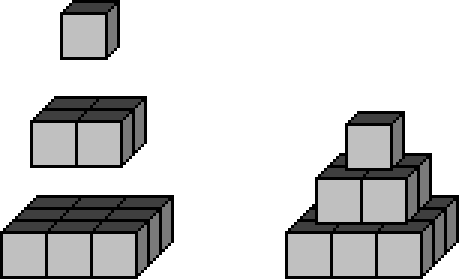
\includegraphics[width=.5\textwidth]{3dimHyper.png}
  \vspace{-0.2cm}
  \caption{A 3-dimensional hyper pyramid with 3 steps consisting of 14 \emph{blocks} in total.}
\end{figure}

\section*{Input}
The input consists of:
\begin{itemize}
	\item one line with a single integer $m$ ($1 \le m \le 10^{16}$) . This integer is the 
	meaningful number the leaders have chosen.	
\end{itemize}


\section*{Output}

If a hyper-step pyramid matching all the requirements exists, output a single line with two
integers $n$ and $s$, the dimension of the pyramid and its number of steps.
If none exists, output \texttt{impossible}. If multiple solutions exist, any will be accepted.
